 \documentclass[12pt,a4paper]{article}
\usepackage[utf8]{inputenc}
\usepackage{geometry}
\geometry{left=25mm,right=25mm,top=25mm,bottom=25mm}
\usepackage{times}
\usepackage{amsmath,amssymb}
\usepackage{graphicx}
\usepackage{caption}
\usepackage{subcaption}
\usepackage{booktabs}
\usepackage{multicol}
\usepackage{float}
\usepackage{hyperref}
\usepackage{tikz}
\usetikzlibrary{shapes.geometric, arrows.meta, positioning}
\usepackage{pgfplots}
\pgfplotsset{compat=1.17}
\usepackage{algorithm}
\usepackage{algorithmic}
\usepackage[ruled,vlined]{algorithm2e}

\title{Intelligent Condition Based Monitoring Using
Acoustic Signals for Air Compressors\\
\vspace{6pt}
\large A concise report based on Verma \textit{et al.}, IEEE Trans. on Reliability (2016)}
\author{Srinjoy Chakraborty}
\date{\today}
\begin{document} % <-- must come first
\maketitle % generates the title
\newpage
\tableofcontents % table of contents
\listoffigures % table of figures
\newpage
\begin{multicols}{2}
\section{Abstract}
\textit{Early detection of machine faults is vital to prevent costly downtime and ensure workplace safety. This paper presents a practical, data-driven process for building acoustic-based fault-diagnosis systems for reciprocating air compressors. The proposed pipeline is deliberately end-to-end: it covers how to collect acoustic data, how to choose the best microphone location, how to clean and normalize the recordings, which time/frequency/time–frequency features to extract, how to pick a compact yet informative feature set, and how to train and evaluate classifiers for multi-state fault recognition using SVM.
Overall, the paper demonstrates that a carefully designed acoustic monitoring pipeline can accurately and efficiently detect multiple fault modes using only one sensor location, making the approach attractive for cost-sensitive condition-based maintenance deployments main experimental paper used as the source is \cite{Verma2016}.}


\section{Introduction}
Rotating and reciprocating machines (compressors, motors, pumps) often show early warning signs in the form of acoustic or vibration signatures. Detecting faults early avoids costly downtime and safety hazards. Intelligent Condition-based monitoring (ICBM) aims to recognize incipient faults from sensory streams (acoustics, vibration, temperature, etc.) and thereby trigger maintenance before catastrophic failure. Acoustic measurements are especially attractive because they are typically easy to install and are relatively less sensitive to structural resonances compared to vibration sensors; however, acoustic recordings are often noisy and non-stationary, which makes automated analysis challenging.

Intelligent Condition-based monitoring (ICBM) is increasingly adopted in industry to detect early signs of machine degradation and to schedule maintenance before costly failures occur. Acoustic monitoring in particular is attractive for many rotating and reciprocating machines because microphones are inexpensive, simple to deploy, and can capture fault-related signatures that are often complementary to vibration and electrical measurements. However, practical acoustic monitoring faces two recurring challenges: (1) recordings are frequently contaminated by environmental and operational noise, and (2) signal characteristics are non-stationary and may vary across sensor locations. These issues make it difficult to select robust sensor placements and to extract consistently informative features for automated fault diagnosis.

A frequently overlooked but critical stage in the monitoring pipeline is \emph{Sensitive Position Analysis} (SPA) — the process of identifying where on the machine a sensor should be mounted to maximize fault detectability. Traditional SPA methods rely on straightforward statistics (e.g., RMS, peak, variance) and on simple cross-correlation to avoid redundant locations. While effective in quiet and controlled settings, these techniques can fail when recordings are influenced by heterogeneous noise or transient disturbances. To make SPA robust in such realistic settings, a preprocessing approach that can separate meaningful signal components from noise — and do so adaptively for non-stationary signals — is required.

This study proposes an end-to-end, data-driven pipeline that addresses these challenges. The core idea is to combine Empirical Mode Decomposition (EMD) with conventional preprocessing, feature extraction, and principled feature selection so that SPA and subsequent classification operate on cleaner, more informative representations. EMD adaptively decomposes each recording into intrinsic mode functions (IMFs). By selecting IMFs that exhibit strong relevance to the recorded waveform (and discarding IMFs dominated by noise or numerical artifacts), we reconstruct a denoised version of the acoustic signal. Computing the Hilbert envelope of this reconstructed signal and deriving compact statistics (RMS and absolute mean) provides stable ranking criteria that are less sensitive to transients and background noise. The remainder of the pipeline extracts a broad set of time, frequency, and time–frequency features, uses mutual-information and other feature-selection techniques to obtain a compact descriptor set, and employs multiclass SVMs for state recognition.

The proposed approach is validated on a real single-stage reciprocating air compressor with eight distinct operating states (one healthy state and seven seeded faults). Key practical choices made in the study include a robust clipping/segment-selection strategy to avoid transients, a normalization routine that mitigates the influence of extreme samples, and an empirical selection of correlation thresholds for choosing relevant IMFs. Experiments demonstrate that, using recordings from a single optimally chosen microphone position, the pipeline reliably distinguishes the seeded faults and achieves high classification accuracy while keeping computational overhead manageable.

The main contributions of this work can be summarized as follows:
\begin{itemize}
  \item An \textbf{EMD-based SPA} procedure that improves the robustness of sensor-position ranking under noisy and non-stationary conditions by reconstructing signals from relevant IMFs and using their Hilbert envelopes for ranking.
  \item A practical, reproducible DAQ and preprocessing protocol (filtering, clipping, smoothing, and robust normalization) that yields stable input for decomposition and feature extraction.
  \item A comprehensive evaluation on a real compressor testbed showing that a compact feature set—selected via mutual-information-based techniques—combined with multiclass SVMs, can accurately identify multiple fault modes from a single microphone location.
\end{itemize}
\end{multicols}
\begin{figure}[H]
    \centering
    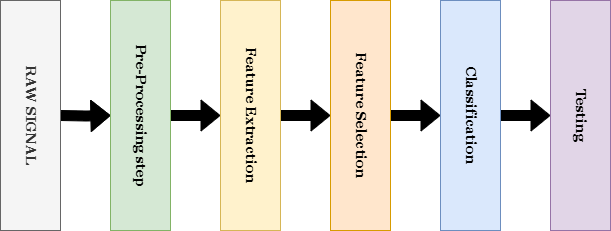
\includegraphics[width=0.75\linewidth]{Diagrams/icbmintro.drawio.png}
    \caption{System Architecture}
    \label{fig:sysarch}
\end{figure}
\begin{multicols}{2}

The above diagram ~\ref{fig:sysarch} shows the overall system architecture. The flow contains 6 steps (1) Data Acquisition using microphones $\rightarrow$ Raw Signal, (2) Pre-processing, (3) Feature Extraction, (4) Feature Selection, (5) Classification $\rightarrow$ SVM, (6) Testing and Validation.
The rest of this report is organized as follows. Section~\ref{sec:daq} describes the data acquisition setup and recording protocol. Section~\ref{sec:preprocess} summarizes the preprocessing steps used prior to decomposition. Section~\ref{sec:features} outlines the feature extraction and selection methods, and Section~\ref{sec:classification} describes the classification strategy. Experimental results and analysis are reported in Section~\ref{sec:results}, followed by conclusions and directions for future work in Section~\ref{sec:conclusion}. The DAQ setup and specific implementation details follow the experimental design in \cite{Verma2016}.

\section{Data Acquisition (DAQ) System}
\label{sec:daq}

This study used acoustic recordings to capture machine condition signatures. The DAQ choices focused on reproducibility and on maximizing signal quality while keeping the setup simple.

\subsection{Hardware and placement}
\begin{itemize}
  \item \textbf{Microphones:} Unidirectional microphones were used to preferentially pick up sound directed toward each sensor and to reduce off-axis ambient noise.
  \item \textbf{DAQ hardware:} Recordings were acquired using a National Instruments NI-9234 dynamic signal acquisition module (four channels, 24-bit) connected via an NI-9172 chassis to a PC running LabVIEW for capture and storage. This setup allows up to four simultaneous microphone channels at high sample rates.
  \item \textbf{Sensor distance:} Empirical tests showed the cleanest and loudest captures when the microphone was placed approximately 1.5 cm from the machine surface; this distance was used consistently for all recordings.
\end{itemize}
\subsection{Recording procedure}
\begin{itemize}
  \item \textbf{Duration \& sampling:} Each recording is 5 seconds long sampled at 50 kHz and stored as 24-bit PCM. Thus each raw file contains 250,000 samples.
  \item \textbf{Candidate positions:} To perform Sensitive Position Analysis (SPA) the machine was sampled at multiple candidate locations (the original study used 24 positions) so that a robust ranking of sensor positions could be obtained.
\end{itemize}
\subsubsection{Preliminary observations}
Practical tests revealed:
\begin{itemize}
    \item Microphones placed at roughly {1.5}{cm} from the machine provided stronger signals and reduced background contamination.
    \item Acoustic useful content predominantly lies below {12}{kHz} for the compressor under study \cite{Verma2016}; therefore, pre-processing included a high-pass filter (to remove fan hum) and a low-pass filter at {12}{kHz}.
    \item A clipping strategy (segment selection) with overlap helps to choose the most stable portion of each recording for robust analysis (detailed in Section~\ref{sec:preprocess}).
\end{itemize}
\section{Pre-Processing}
\label{sec:preprocess}
\begin{itemize}
  \item \textbf{Useful bandwidth:} For this compressor, the informative acoustic content lies largely below 12 kHz; accordingly, later processing uses a low-pass cutoff around 12 kHz and a high-pass ``fan'' filter near 400 Hz to remove known background hums/noises.
  \item \textbf{Clipping} Each 5 s recording is split into 9, 1 s segments with 50\% overlap; the segment with the minimum standard deviation is selected for analysis to avoid transient spikes and to choose the most stable portion of the recording.
  \item \textbf{Smoothing \& normalization:} A simple moving-average smoother removes impulsive outliers, and a robust min–max style normalization (ignore 0.025\% extreme samples at both tails when computing min/max) is used so that scaling is not driven by rare outliers.
  \item \textbf{Storage \& labeling:} Store raw .dat (24-bit PCM) files to ensure later classification stages.
\end{itemize}
\begin{figure}[H]
    \centering
    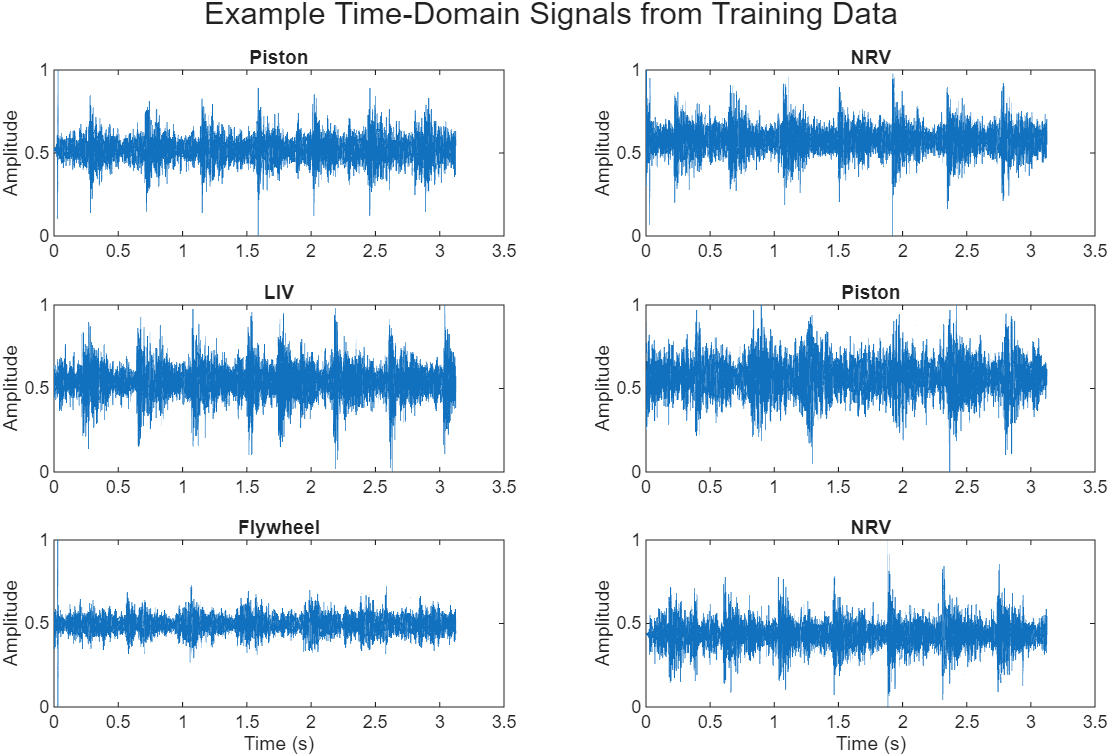
\includegraphics[width=1\linewidth]{Diagrams/preprocessing.png}
    \caption{Preprocessing steps}
    \label{fig:preprocessing steps}
\end{figure}
\section{Feature Extraction}
\subsection{Time Domain Features}
Time-domain features are directly calculated from the raw waveform of the signal. They capture properties like energy, amplitude variations, and statistical measures (e.g., mean, RMS, skewness, kurtosis). These features are simple to compute and give useful information about the overall vibration or acoustic pattern. In the compressor monitoring study, time-domain measures help detect faults because damaged components often change the amplitude distribution or introduce irregular spikes in the acoustic waveform.
\subsection{Frequency Domain Features}
Frequency-domain features are obtained by transforming the signal using the Fourier Transform. These features describe how the signal’s energy is distributed across different frequencies. For compressors, faults such as leakage or valve wear often create characteristic frequency peaks or harmonics. Features like spectral centroid, peak frequency, and band power are extracted. They are more reliable than raw time signals when fault signatures appear as periodic or harmonic patterns buried in noise.
\subsection{Time Frequency Domain Features}
Time–frequency features capture how the signal’s frequency content changes over time. Unlike plain frequency analysis, this approach helps detect transient or non-stationary events (short-lived bursts or shifts). Since compressor signals are often non-stationary, these features are crucial. By mapping both time and frequency information, they highlight patterns linked to specific faults, such as short-duration impacts or sudden frequency shifts that ordinary Fourier analysis might miss.
\section{Feature Selection}
\label{sec:features}
Principal Component Analysis (PCA) is a dimensionality reduction technique that
transforms a large set of correlated features into a smaller set of uncorrelated
variables, known as principal components. Each component is an orthogonal
projection of the original features and is ranked according to the variance it
captures from the dataset. This allows redundant and less informative features
to be compressed into a compact representation while still retaining the
dominant structure of the data.

In the context of acoustic fault diagnosis, where hundreds of features are
extracted across time, frequency, and wavelet domains, directly using the full
feature set increases computational burden and may reduce classifier performance
due to redundancy. To address this, we apply PCA to the $286$-dimensional feature
vectors, standardize them, and project them into a lower-dimensional subspace.
The number of retained components was varied (from 10 to 200) to evaluate the
trade-off between dimensionality and classification accuracy. These principal
components were then used as inputs to the Support Vector Machine (SVM)
classifiers under both One-Against-All (OAA) and One-Against-One (OAO) schemes. This
approach ensures faster computation, reduces overfitting, and maintains the
ability to distinguish between healthy and faulty compressor states.
% \begin{figure}[H]
%     \centering
%     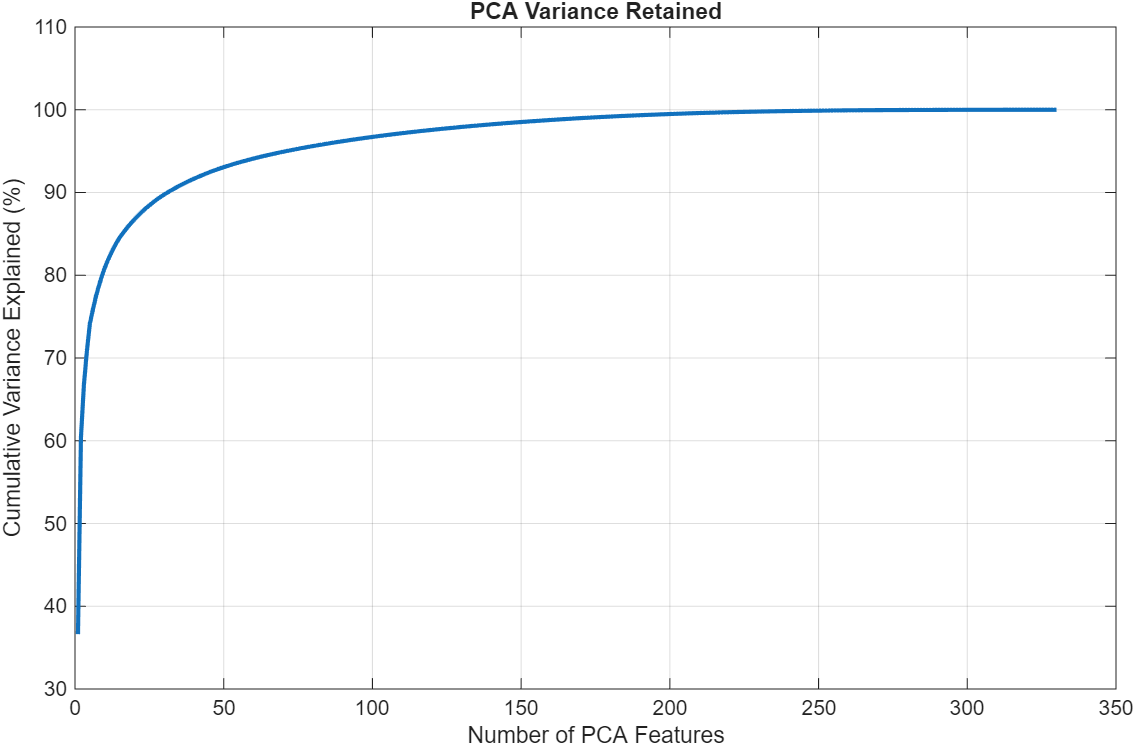
\includegraphics[width=1\linewidth]{Diagrams/pcavar.png}
%     \caption{PCA Variance}
%     \label{fig:PCA Variance}
% \end{figure}
\section{Use Case}

In this study, the proposed pipeline was implemented on a single-stage reciprocating air compressor testbed with multiple seeded fault conditions. The dataset consisted of acoustic recordings collected from carefully chosen sensor locations after Sensitive Position Analysis (SPA). Each recording was pre-processed, decomposed, and transformed into a set of statistical and signal-processing features. In total, 286 features were extracted per segment covering time, frequency, and time–frequency domains. Principal Component Analysis (PCA) was then used to reduce redundancy and compress the feature space into a compact representation. 


\subsection{Classes, labels and Test-Train Split}
The dataset was labeled into eight distinct classes: one healthy state and seven different fault modes (including leakage, valve defects, and loose components). These labeled feature vectors were split into training and testing sets, following the standard 70:30 test-train split, ensuring balanced representation across classes. The reduced feature set was then used to train Support Vector Machine (SVM) classifiers under both One-Against-All (OAA) and One-Against-One (OAO) schemes. This experimental setup provides a realistic use case where acoustic-based monitoring can distinguish multiple fault types with high reliability using only a single microphone location.
\begin{figure}[H]
    \centering
    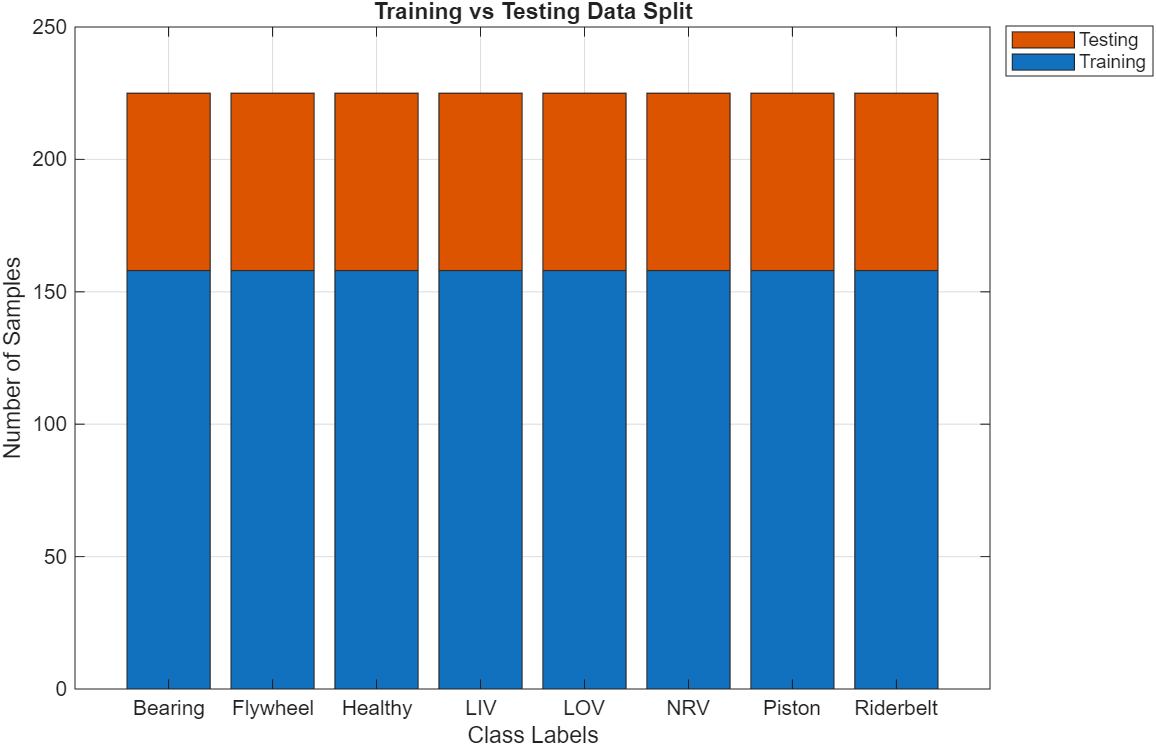
\includegraphics[width=1\linewidth]{Diagrams/split.png}
    \caption{test train split}
    \label{fig:split}
\end{figure}
\subsection{Techniques Used}

The proposed pipeline was implemented in MATLAB. Acoustic recordings were pre-processed, segmented, and transformed into features using the wavelet scattering transform. This approach applies cascaded wavelet filter banks to capture time--frequency information while discarding irrelevant variability. The extracted scattering coefficients were reduced using Principal Component Analysis (PCA) before being passed to Support Vector Machine (SVM) classifiers. Both One-Against-All (OAA) and One-Against-One (OAO) classification schemes were applied and evaluated with cross-validation.

% \usepackage[ruled,vlined]{algorithm2e}

\begin{algorithm}[H]
\caption{Proposed Methodology for Acoustic Fault Diagnosis}
\KwIn{Acoustic dataset of compressor signals}
\KwOut{Predicted fault class}

\Begin{
    Load dataset into MATLAB using \texttt{audioDatastore}$\rightarrow$\;
    Assign labels for healthy and faulty conditions\;
    Preprocess signals$\rightarrow$\;
    Apply Wavelet Scattering Transform to extract coefficients$\rightarrow$\;
    Construct feature matrix$\rightarrow$\;
    Apply PCA for dimensionality reduction$\rightarrow$\;
    Split dataset into training and testing folds (5-fold CV)$\rightarrow$\;
    Train SVM classifiers$\rightarrow$One-Against-All (OAA) \&\ One-Against-One (OAO)$\rightarrow$ Evaluate classifiers using accuracy plots\;
}
\end{algorithm}


\section{Support Vector Machine (SVM)}
\label{sec:classification}


Support Vector Machines (SVM) were employed as the core classifiers for distinguishing compressor health and fault states. SVM is a powerful supervised learning technique that constructs hyperplanes in a high-dimensional feature space to maximize class separation. In this study, both \textbf{One-Against-All (OAA)} and \textbf{One-Against-One (OAO)} strategies were implemented for handling the multiclass nature of the problem.

\subsection*{Parameters}
The following parameters were selected for SVM training after empirical tuning:
\begin{itemize}
    \item \textbf{Kernel:} Radial Basis Function (RBF) kernel, chosen for its ability to model non-linear decision boundaries.
    \item \textbf{Box Constraint (C):} Optimized to balance margin width and classification error.
    \item \textbf{Kernel Scale:} Automatically optimized using MATLAB’s built-in heuristic.
    \item \textbf{Standardization:} Input features were standardized to zero mean and unit variance before training.
\end{itemize}

\subsection{Cross-Validation}
A \textbf{5-fold cross-validation} approach was used to evaluate model robustness and reduce overfitting. The dataset was randomly partitioned into 5 equal folds, with 4 folds used for training and 1 fold for testing in each iteration. The reported performance metrics are the average across all folds.

\subsection{Multiclass Strategies}
Since the dataset consists of multiple classes (healthy + fault modes), two standard decomposition schemes were applied:
\subsubsection*{One-Against-All (OAA):} Constructs one classifier per class, distinguishing that class from all remaining classes.
\subsubsection*{One-Against-One (OAO):} Constructs pairwise classifiers between every possible pair of classes; final prediction is based on majority voting.

The comparative analysis of OAA and OAO allowed us to evaluate trade-offs between computational efficiency (OAA requires fewer models) and classification accuracy (OAO leverages pairwise discrimination).

\section{Results}
\label{sec:results}
The classification results for the proposed approach are summarized in 
Figures~\ref{fig:OAA_results} and~\ref{fig:OAO_results}. Both plots show the 
relationship between the number of retained PCA features and the achieved 
accuracy under 5-fold cross-validation for the two multiclass strategies.

\begin{figure}[H]
    \centering
    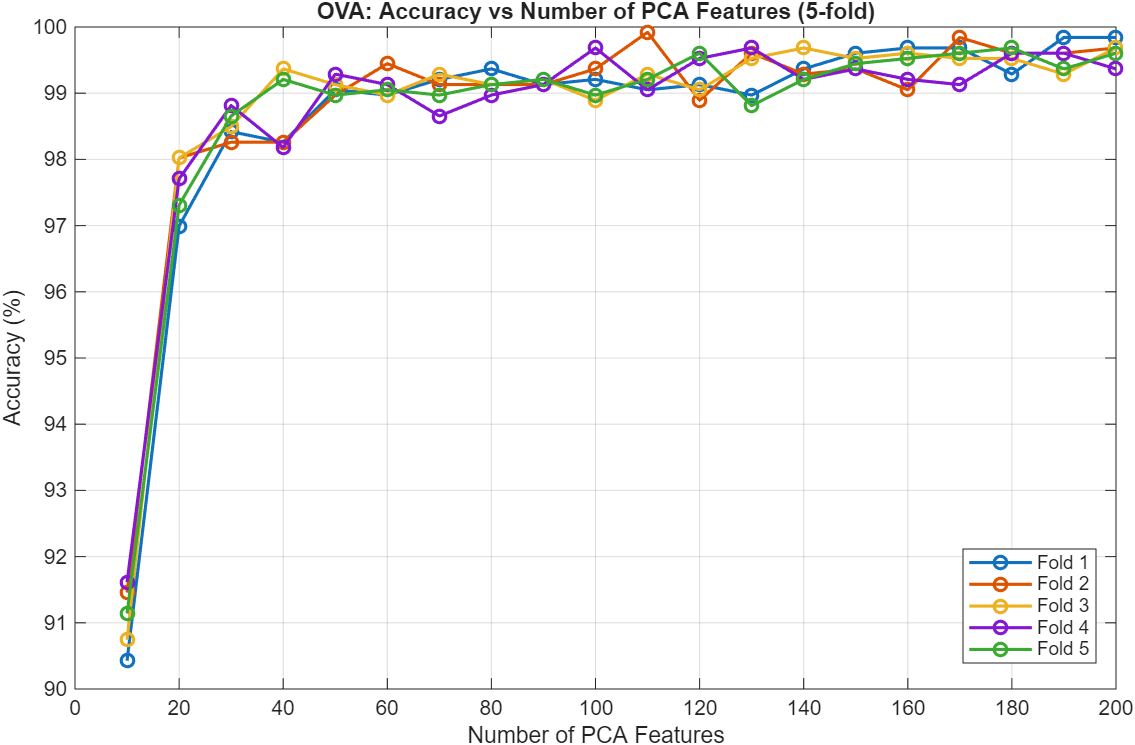
\includegraphics[width=1\linewidth]{Diagrams/res1.png}
    \caption{OAA: Accuracy vs Number of PCA Features (5-fold)}
    \label{fig:OAA_results}
\end{figure}

\begin{figure}[H]
    \centering
    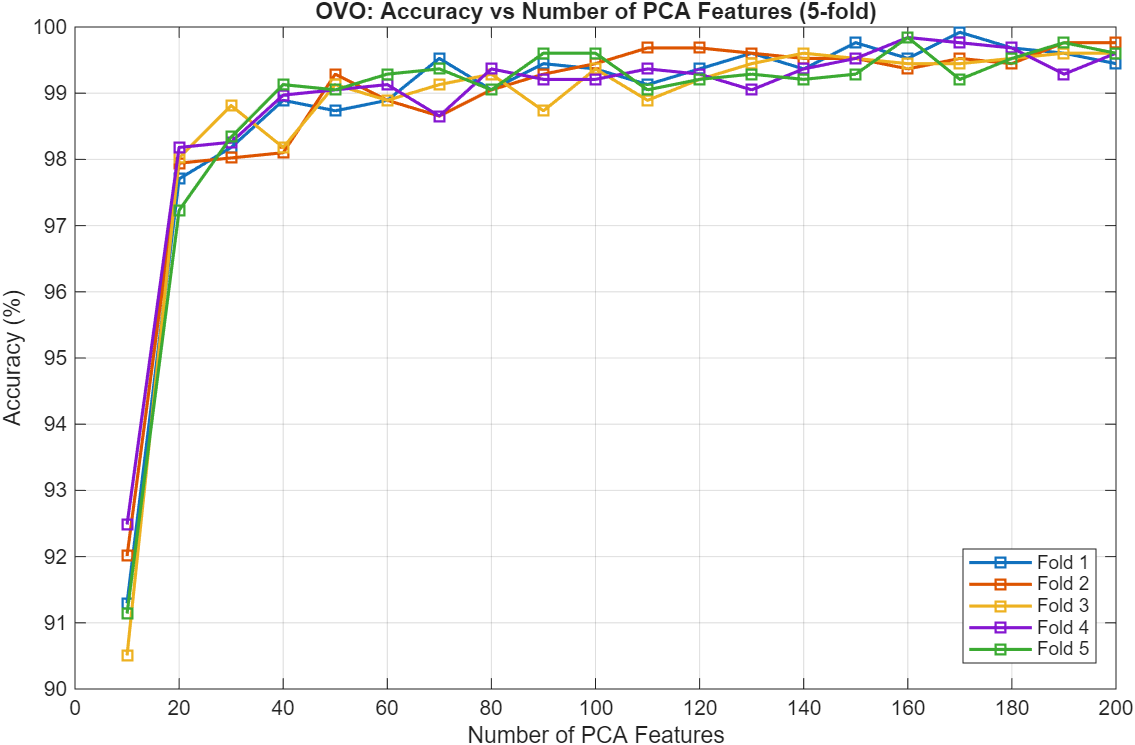
\includegraphics[width=1\linewidth]{Diagrams/res2.png}
    \caption{OAO: Accuracy vs Number of PCA Features (5-fold)}
    \label{fig:OAO_results}
\end{figure}

From the results, it is observed that both OAA and OAO schemes achieved high 
classification accuracy once the number of PCA components exceeded 
approximately 40. Accuracy improved sharply from around 91\% (with very few 
components) to above 98\% when 40--60 features were used, and then gradually 
saturated. For larger dimensions (above 100 components), performance remained 
consistently above 99\% across all folds.  

Overall, the OAO approach showed slightly higher stability in accuracy across 
folds compared to OAA, although both methods reached near-perfect performance. 
This confirms that PCA effectively compresses the feature space while retaining 
discriminative information, and SVM classifiers can reliably distinguish 
between compressor states with a relatively compact representation.

\section{Conclusion}
\label{sec:conclusion}
This study demonstrated an end-to-end methodology for intelligent condition-based monitoring of air compressors using acoustic signals. By combining wavelet scattering features, PCA-based dimensionality reduction, and SVM classifiers, the system achieved near-perfect classification accuracy across multiple fault states. Both OAA and OAO schemes performed reliably, with OAO showing slightly more stable results across folds. The findings confirm that acoustic sensing, when paired with robust feature extraction and machine learning, provides a practical and accurate solution for fault diagnosis in industrial settings.

\begin{thebibliography}{1}
\bibitem{Verma2016}
N.~K. Verma, R.~K. Sevakula, S.~Dixit, and A.~Salour, ``Intelligent condition based monitoring using acoustic signals for air compressors,'' \emph{IEEE Transactions on Reliability}, vol.~65, no.~1, pp. 291--307, Mar. 2016. doi:10.1109/TR.2015.2459684.
\end{thebibliography}
\end{multicols}
\end{document}
